\chapter{Proteus et nos outils d'analyse}
\label{chap:methodes}

Il existe plusieurs logiciels de CPD. Parmi les plus connus, on peut citer ORBIT (Optimisation of Rotamers By Iterative Techniques) \cite{Dahiyat96}, OSPREY (Open Source Protein REdesign for You) \cite{Gainza13}, Rosetta (le CPD n'est qu'une partie des fonctionnalités proposées par cette suite logicielle) \cite{Kuhlman03} et Proteus \cite{Simonson13,Polydorides16}. Proteus est le logiciel développé par notre équipe au laboratoire de Biochimie de l'École Polytechnique. Dans ce chapitre, nous détaillons quelques points importants de notre logiciel.  

\section{Un modèle fondé sur la Physique}
\label{sec:Phy}
Proteus se base sur la théorie de la mécanique statistique pour formaliser les problèmes auxquels il s'attaque et pour guider sa sélection de meilleures séquences-conformations. À partir d'un postulat fondamental et de l'hypothèse ergodique, la mécanique statistique \og redécouvre \fg la thermodynamique classique et en plus, établit une relation à l'équilibre entre l'énergie d'un état $i$ d'un système et la probabilité que le système soit en $i$ par la probabilité de Boltzmann, voir l'équation \vref{eq:Boltzmann}. Ainsi, si l'on considère deux états A et B d'un système S à l'équilibre, le ratio des probabilités que S soit dans l'état A ou dans l'état B s'exprime en fonction de la différence entre l'énergie de A et de B. Pour le CPD, l'énergie qui est pertinente est celle qui prend en compte l'énergie interne de la protéine, mais aussi son environnement aqueux moyen. Il s'agit donc d'une énergie libre de Gibbs $G$. De plus, on prend la différence entre états replié et déplié.

Nous introduisons alors un cycle thermodynamique pour définir la stabilité d'une séquence-conformation, voir figure \ref{fig:cycleThermo}. Le cycle considère la stabilité de deux séquences A et B. La transformation de A en B correspond aux deux flèches horizontales. Le dépliement est figuré par les deux flèches verticales. La différence de stabilité entre les deux séquences correspond à la différence d'énergie libre des transformations horizontales (comme verticales). On a alors la différence: 

\begin{equation}
  \label{deltaG}
\Delta \Delta G = (G(S^P_B)- G(S^P_A)) - (G(S^D_B)- G(S^D_A))
\end{equation}  
avec respectivement $S^P_A$, $S^P_B$, $S^D_B$ et $S^D_B$, le système avec la séquence $A$ repliée, $B$ repliée, $A$ dépliée et $B$ dépliée. Maximiser la stabilité d'une séquence-conformation $B$ correspond alors à minimiser $\Delta \Delta G$.

   \begin{figure}[!htbp]
     \centering
     \begin{tabular}{c}
       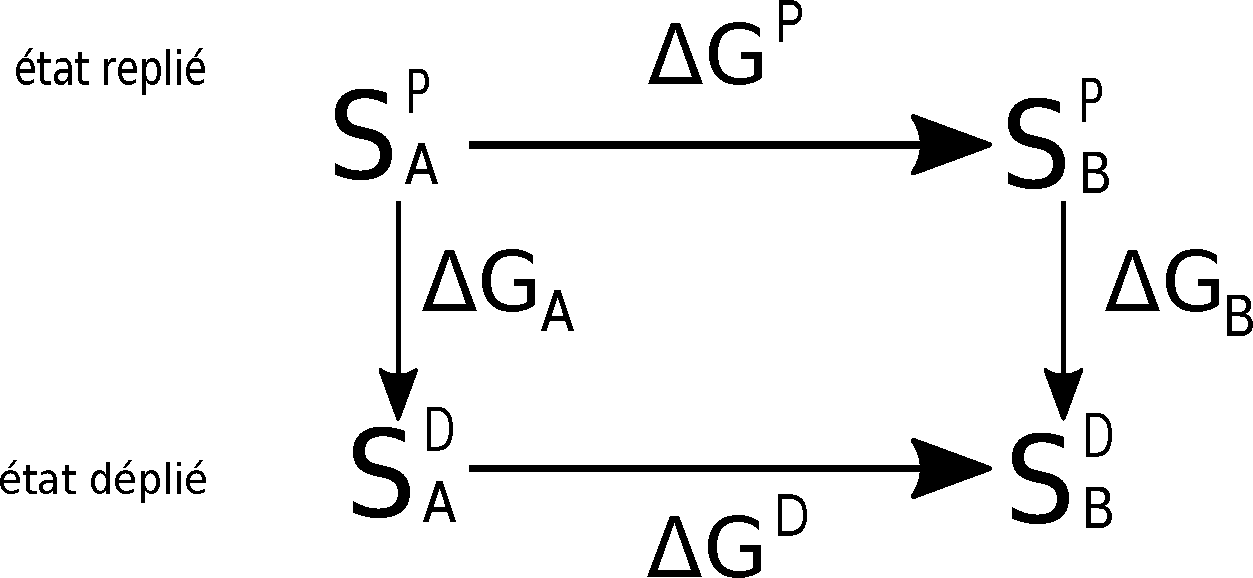
\includegraphics[width=6cm]{figure/cycleThermo.pdf} \\
     \end{tabular}
     
     \caption{Cycle thermodynamique qui définit la stabilité relative de deux séquences-conformations $S_A$ et $S_B$.}
\label{fig:cycleThermo}
   \end{figure}


Nous faisons des simulations avec deux mouvements élémentaires possibles: un changement de rotamère dans la sequence repliée courante et une mutation qui consiste à modifier le type de la chaîne latérale à une position $i$ tirée au hasard. Le changement d'énergie $\Delta E_{m_1}$ associé à un changement de rotamère $r_i$ vers $r'_i$ est:
\begin{equation}
\Delta E_{m_1}= E^f(...,t_i,r'_i,...) - E^f(...,t_i,r_i,...)     
\end{equation}   
avec $E^f$ l'énergie de l'état replié. Pour le changement d'énergie $\Delta E_{m_2}$ d'une mutation de $t_i$ vers $t'_i$, nous appliquons l'equation \ref{deltaG} à la séquence-conformation avant et après la mutation:    
\begin{equation}
\Delta E_{m_2}= (E^f(...,t'_i,r'_i,...) - E^f(...,t_i,r_i,...)) - (E^u(t'_i) - E^u(t_i))     
\end{equation}   
avec $E^f$ l'énergie de la l'état replié et $E^u$ l'énergie de l'état déplié. Cela peut s'interpréter comme le changement à la position $i$ de $t_i$ vers $t'_i$ dans l'état repliée et du changement inverse $t'_i$ vers $t_i$ dans l'état déplié. Comme nos simulations Monte Carlo respectent le schéma de Métropolis, les séquences-conformations sont visitées suivant leur probabilité de Boltzmann. Ainsi le ratio des populations de deux séquences-conformations obtenues est fonction de leur stabilité relative. 
   

\section{Organisation générale}

Proteus est constitué de trois parties:
\begin{itemize}
\item une version modifiée de Xplor, qui fournit plusieurs modèles de solvant et plusieurs fonctionnalités spécifiques au CPD. Xplor est un programme de simulation moléculaire \cite{Xplor}, disponible en téléchargement sur le site de l'université de Yale. Les modifications CPD sont disponibles sur notre site Web. 
\item un ensemble de scripts Xplor, qui pilote le calcul de la matrice d'énergie. 
\item un programme écrit en C, que nous appelons \og proteus\fg qui explore l'espace des séquences-conformations
\end{itemize}
Proteus est flexible et largement configurable. Il permet l'utilisation de plusieurs champs de force, de plusieurs modèles de solvant, et de plusieurs librairies de rotamères. La partie en C, proteus, propose plusieurs algorithmes d'exploration comme le MSD, MC ou REMC. Le programme proteus permet de diviser le système en plusieurs groupes ou d'en dupliquer une partie. Ceux-ci pouvent alors être combinés dans une fonction de score basée sur la fonction d'énergie physique afin de favoriser la stabilité de certains sous-ensembles du système ou certaines affinités. Plusieurs succès ont déjà était obtenue avec Proteus par exemple le redesign de la tyrosyl-ARNt synthétase \cite{Simonson16}, les calculs de $pK_a$ \cite{Villa17} ou la création de nouveaux domaines PDZ \cite{Mignon17}.

Proteus autorise le choix de plusieurs fonctions d'énergie. La plus simple \og MMCASA \fg combine la mécanique moléculaire pour la protéine et un modèle de solvant implicite CASA (voir  \vref{sub:CASA}). Deux types \og MMGBSA \fg sont également possibles, dans lesquels le traitement du solvant est effectué par un modèle de Born Genéralisé. Nous détaillons les points importants de Proteus dans la suite.

\section{Décomposition par paires de la fonction d'énergie}
Une fonction d'énergie décomposable par paires permet de réduire le calcul de l'énergie d'une séquence-conformation à une somme d'énergies précalculées. Cependant, les termes GB et SA ne sont pas rigoureusement décomposables par paires. Il faut alors introduire de nouvelles approximations pour permettre cette décomposition. Voyons dans la suite comment ces problèmes sont résolus dans Proteus.
\subsection{Décomposition du terme de surface}
\label{sub:surpairwise}

Le terme surfacique présenté en \vref{eq:SA}, se définit comme:
\begin{equation}
E_{solv}^{surf} = \sum_i \sigma_{t_i} A_i 
\end{equation}
avec $A_i$ la surface accessible au solvant de l'atome $i$, et $\sigma_{t_i}$ un coefficient d'hydrophobicité de l'atome $i$.
Ce terme n'est pas décomposable par paires de résidus, parce que la surface d'une première chaîne latérale enfouie par une deuxième peut aussi être enfouie par une troisième, voir la figure \ref{fig:intersurf}.

   \begin{figure}[!htbp]
     \centering
     \begin{tabular}{c}
       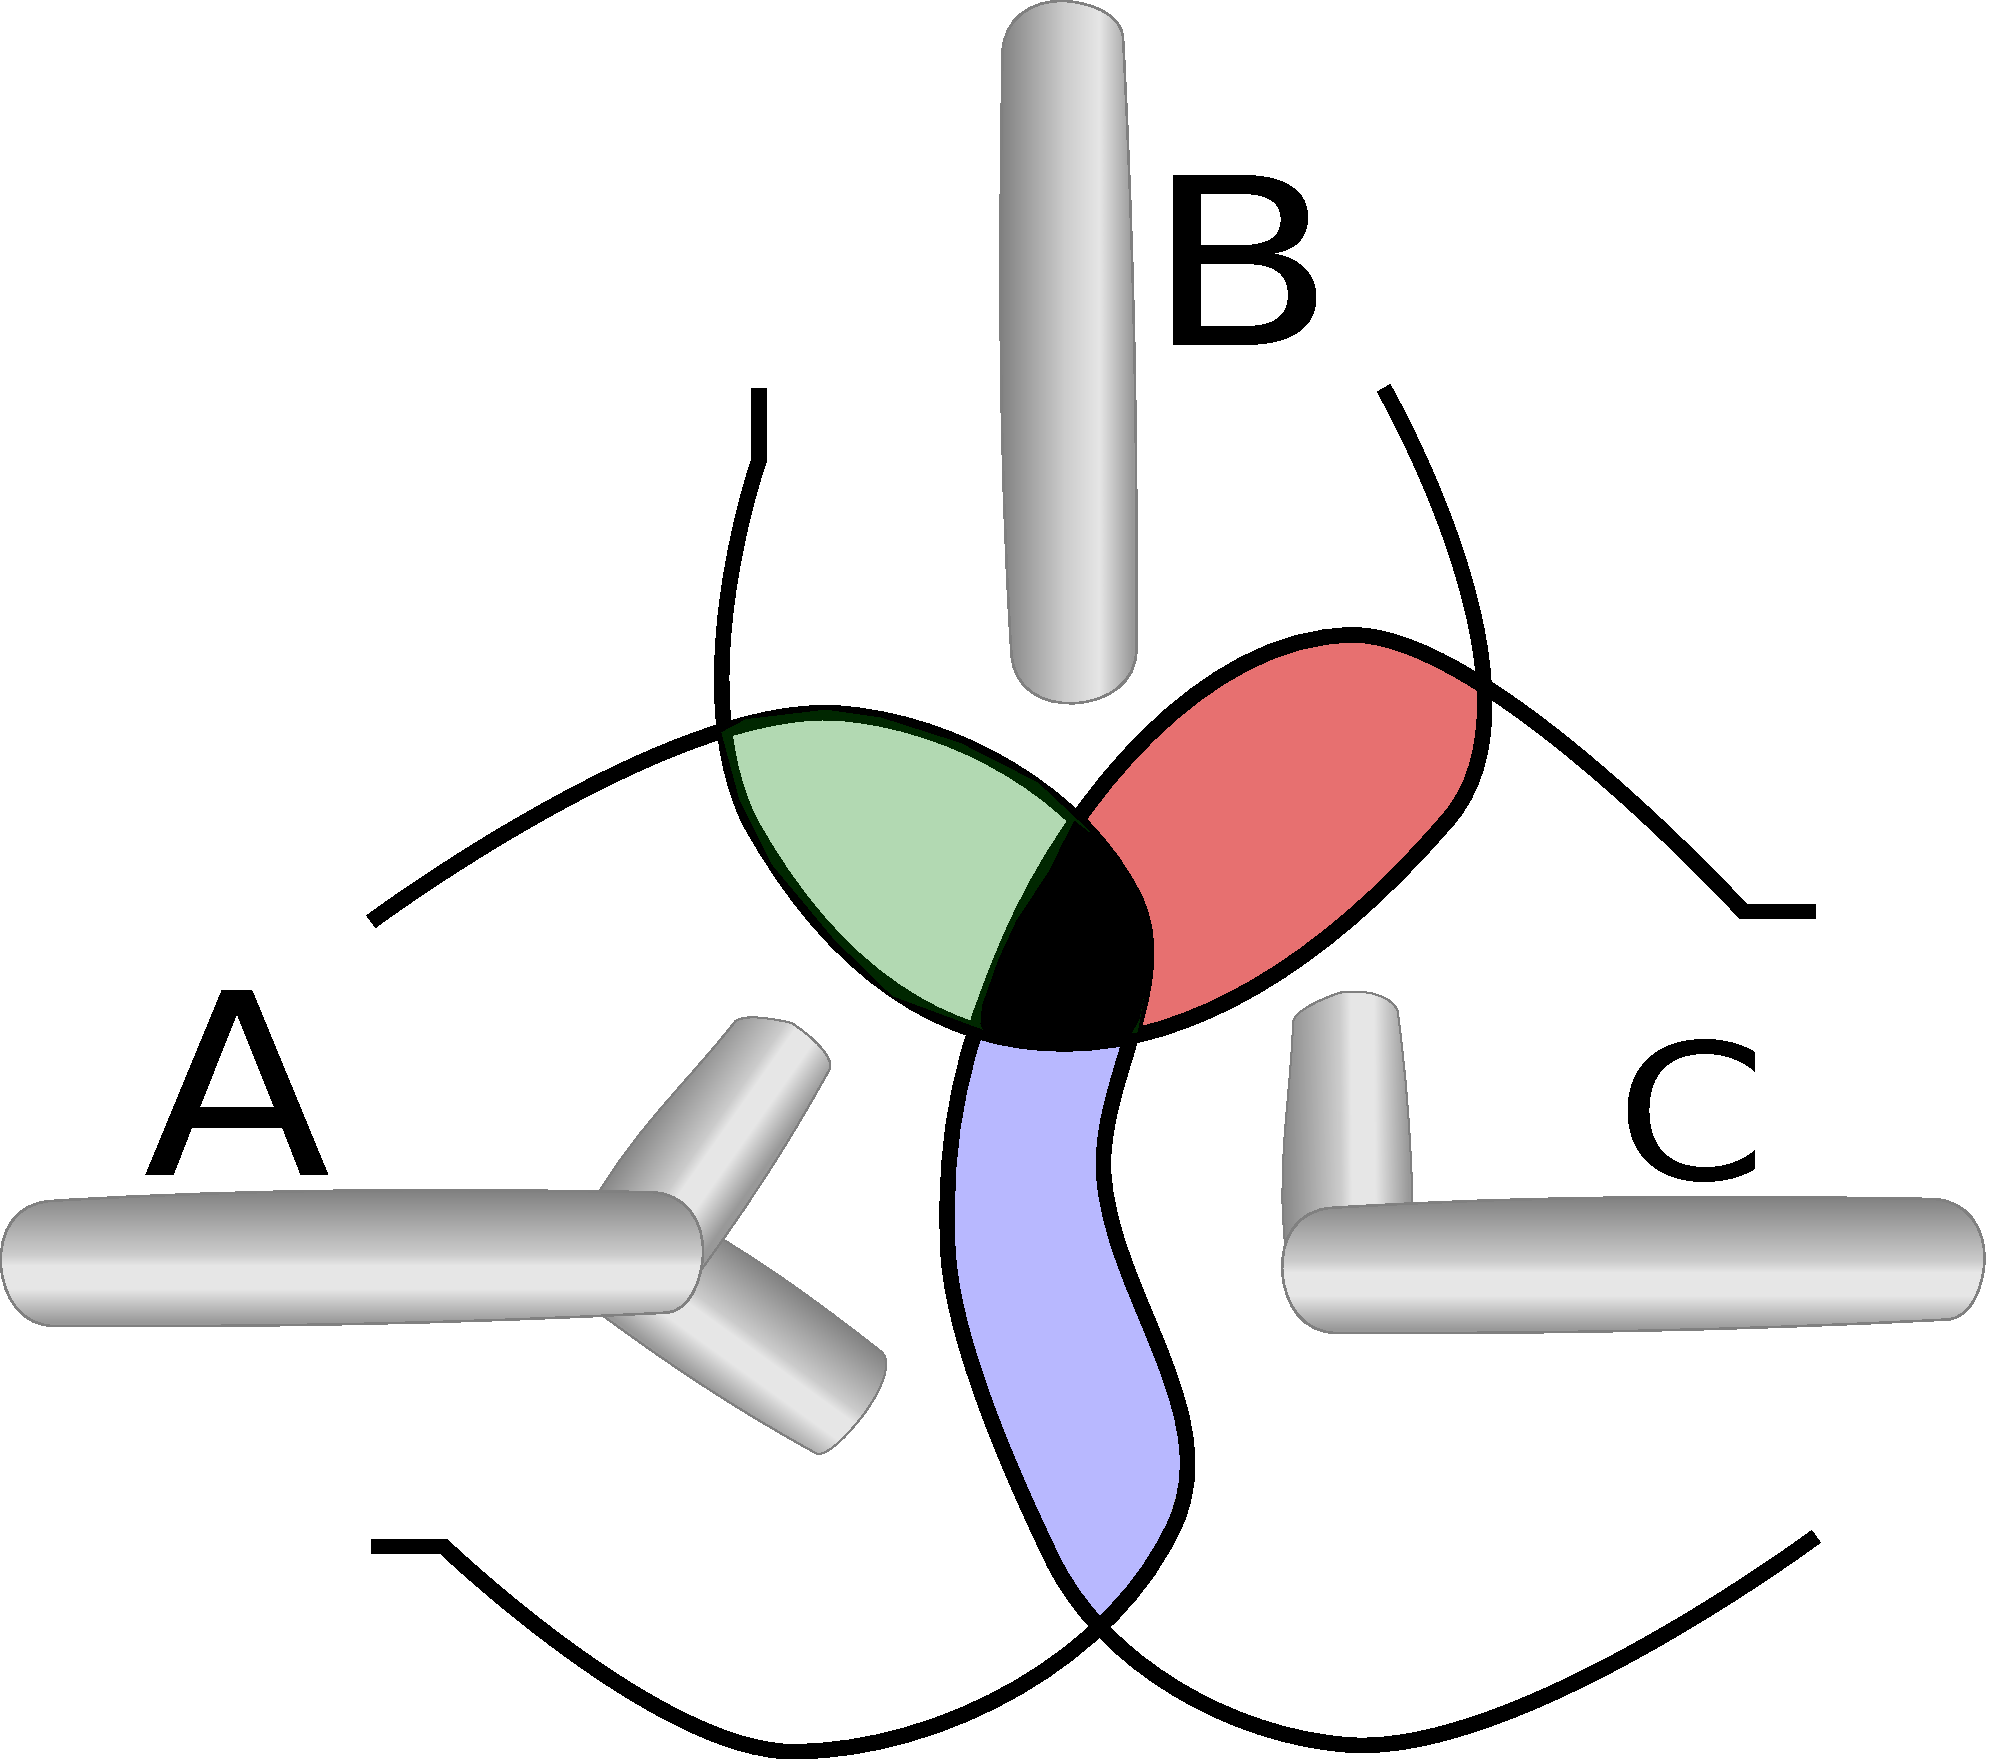
\includegraphics[width=8cm]{figure/intersurface.pdf} 
     \end{tabular}
     
     \caption{\textbf{Une représentation de la surface accessible de trois résidus.} Les résidus A et B réduisent mutuellement leur surface exposée au solvant: c'est la zone verte. De même pour B, C : la zone rouge et  A, C, la zone bleue. Un calcul par paires de résidus naïf surestime la surface accessible en comptant deux fois la zone noire. }
\label{fig:intersurf}
   \end{figure}


Pour rendre ce terme décomposable, nous utilisons la méthode de Street et al. \cite{Street98} dans laquelle la surface enfouie d'une chaîne latérale est calculée à partir d'une somme sur les groupes voisins. Puis pour chaque groupe voisin, la surface de contact avec notre chaîne est calculée indépendamment des autres groupes. Ces surfaces de contact sont sommées et un facteur de réduction est appliqué mimant l'élimination des doubles comptages. Des travaux précédents effectués dans notre laboratoire ont montré qu'un facteur de 0,65 fonctionne bien \cite{Lopes07,Gaillard14}.   


\subsection{\og Native Environnement Approximation\fg (NEA)}

Dans le terme GB de l'énergie de solvatation, le rayon de solvatation $b_i$ approxime la distance de l'atome $i$ à la surface de la protéine. C'est une fonction de la position de tous les atomes de la protéine. Pour que ce rayon soit décomposable par paire, Proteus implémente l'approximation  NEA qui est présentée à  la section \vref{NEA}. Dans cette approche, le rayon de solvatation $b_i$ de chaque groupe (backbone, chaîne latérale ou ligand) est calculé une fois pour toutes en utilisant pour chacun de ses rotamères la structure native pour les autres groupes.

\subsection{\og Fluctuating Dielectric Boundary\fg (FDB)}
\label{sec:FDB}
Une nouvelle approximation GB a récemment été introduite dans Proteus \cite{Villa17}, toujours avec l'objectif de rendre ce terme décomposable par paires. Elle exploite le fait que dans le GB, l'environnement diélectrique d'une paire de résidus est complètement caractérisé pour un petit ensemble de rayons de solvatation d'atomes. Ces rayons sont eux-mêmes sommes de paires sur les atomes de la protéine \cite{Hawkins95}, \cite{Schaefer96}. La méthode s'appelle Fluctuating Dielectric Boundary\fg ou FDB et comporte deux étapes.

La première consiste à définir un rayon de solvatation $B_I$ pour chaque résidu $I$ de la protéine. On définit une énergie propre à chaque paire de résidus $I$, $J$ par la somme suivante:
\begin{equation}
  E_{IJ}^{self} \stackrel{def}{=} \sum_{i\in I,j\in J} E_{ij}^{self}
\end{equation}
puis l'énergie propre d'un résidu $I$:

\begin{equation}
  E_I^{self} \stackrel{def}{=} \sum_J E_{IJ}^{self}
\end{equation}
Alors le rayon de solvatation moyen $B_I$ est défini par:
\begin{equation}
  E^{self}_I \stackrel{def}{=} \tau \sum_{i \in I} \frac{q_i^2}{2 B_I}
\end{equation} 
avec $ \tau = \frac{1}{\epsilon_p} - \frac{1}{\epsilon_s}$, $q_i$ la charge de l'atome $i$. Nous avons
\begin{equation}
\left( \sum_{i \in I} q_i^2 \right) \frac{1}{B_I} = \sum_{i \in I} \frac{q_i^2}{b_i}
\end{equation}
$B_I$ est donc la moyenne harmonique des $b_i$ pondérés par les charges au carré. Il est alors possible de définir la contribution $g_{IJ}$ de la paire de résidus $I$ et $J$ à l'énergie $\Delta G_{elec}$, par:
\begin{equation} 
g_{IJ} = \sum_{i \in I, j \in J} \tau q_i q_j \left( r_{ij}^2 + B_I B_J \exp[-r_{ij}^2/4 B_I B_J] \right)^{-1/2}
\label{eq:screen}
\end{equation}
Pour $I=J$, on exclue les termes $i=j$. On peut noter qu'aux distances fixes $r_{ij}$, et avec $B=B_IB_J$, $g_{IJ} (B)$ varie faiblement en fonction de $B$. Archontis et Simonson \cite{Archontis05}, proposent d'approximer cette fonction par:
\begin{equation}
  \label{eq:approx}
g_{IJ}(B) \approx c_1^{IJ} + c_2^{IJ} B + c_3^{IJ} B^2 + c_4^{IJ} B^{-1/2} + c_5^{IJ} B^{-3/2} 
\end{equation}
Les coefficients $c_n^{IJ}$ peuvent être précalculés et stockés dans la matrice d'énergie, puisque les distances $r_{ij}$ ne sont pas des variables pour un couple de chaînes latérales $I$, $J$ et un choix de rotamères donnés. Pour une conformation donnée, le calcul de l'énergie GB à l'aide de l'approximation \ref{eq:approx} est maintenant décomposable par paires.

\section{La matrice d'énergie}

Proteus utilise un backbone fixe, un espace discret de rotamères et une fonction d'énergie décomposable par paires. Ces trois éléments permettent de précalculer toutes les énergies d'interactions possibles. À cet ensemble d'interactions, il faut ajouter les interactions des résidus avec le backbone, pour chacun des rotamères possibles, pour constituer un ensemble complet de valeurs énergétiques. Cet ensemble  permet d'obtenir rapiement la valeur de la fonction d'énergie pour chaque séquence-conformation. Cet ensemble peut être organisé sous la forme d'une matrice symétrique dans laquelle chaque couple de positions dans la chaîne polypeptidique apparaît avec sa multiplicité de couples de rotamères possibles, voir la figure \ref{fig:matener}.      

   \begin{figure}[!htbp]
     \centering
     \begin{tabular}{c} 
       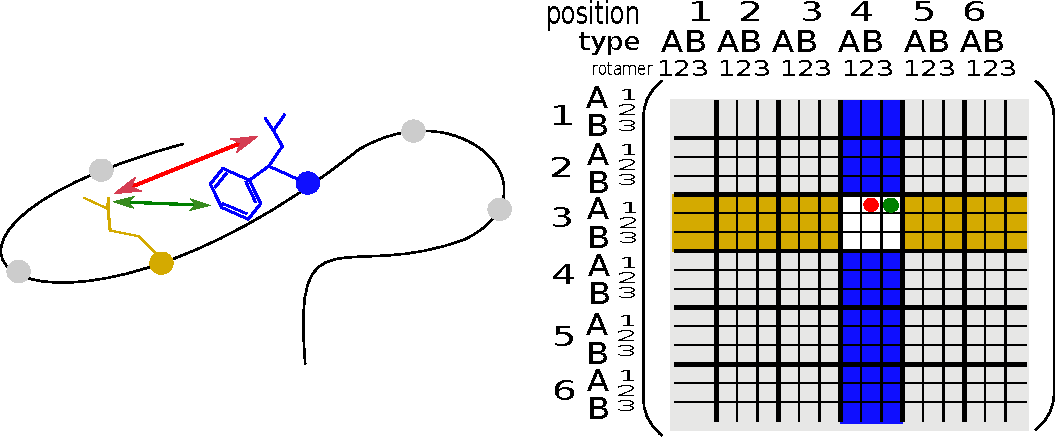
\includegraphics[width=15cm]{figure/matrice.pdf}
       \label{Graph:mat_ener}
     \end{tabular}
     
     \caption{\textbf{La matrice d'énergie.} Cet exemple montre un polypeptide de 6 résidus, chaque position possède 2 types d'acides aminés possibles et 3 rotamères possibles (2 pour le type A et 1 pour le type B). La matrice organise toutes les interactions de paires de chaînes latérales possibles. Les interactions de la bande jaune de la matrice impliquent le résidu numéro 3, celles de la bande bleue impliquent le résidu numéro 4. Les points rouge et vert correspondent aux interactions notées respectivement par les flèches rouge et verte à gauche.}
\label{fig:matener}
   \end{figure}
   
\subsection{Les énergies de l'état déplié}
Notre expression de la stabilité relative de deux séquences-conformations se base sur la différence d'énergies $\Delta \Delta G$ entre l'état replié de la protéine et un état déplié. Nous avons donc besoin d'attribuer une énergie à l'état déplié. Proteus utilise une définition indépendante de la structure, telle que:
\begin{equation}
E^u(S) = \sum_i^N E^u_{t_i}  
\end{equation}
avec $E^u_{t_i}$ l'énergie du type d'acide aminé $t_i$. Ces énergies sont prises en entrée dans Proteus et leur détermination en amont doit être fonction du système étudié. Nous détaillerons dans le chapitre \ref{chap:PDZ} plusieurs méthodes dont de nouvelles et plusieurs exemples de détermination qui seront exploités et évalués.

\subsection{Déroulement de la construction de la matrice}
\label{sub:matrix}
Dans la suite, on appelle position active une position pour laquelle tous les types d'acides et tous les rotamères de chaque type d'acide aminé sont autorisés au cours de l'exploration. Lorsqu'une position n'est pas active, le type de l'acide aminé de la position est fixé. Si les rotamères de la chaîne latérale ne sont pas fixés, on dit que la position est inactive. Si la position n'est pas active et qu'en plus la conformation est fixée, on dit que la position est gelée.

Le calcul de la matrice d'énergie est exécuté à l'aide du programme Xplor \cite{Xplor}. À partir d'un fichier PDB, une série de scripts Xplor commence par préparer le système, qui peut contenir un ligand. Le déroulement est le suivant:

\begin{enumerate}[leftmargin=*]
\item L'utilisateur configure l'exécution. Il détermine:
\begin{itemize}
\item un champ de force (AMBER ff99SB, CHARMM19, CHARMM22, OPLS sont supportés.)
\item un traitement du solvant parmi CASA, GB/NEA, GB/FDB
\item un jeu de coefficients $\sigma_i$ pour la pondération de la surface accessible au solvant
\item un jeu d'énergies dépliées $E^u_{t_i}$  
\item les résidus autorisés à muter
\item les résidus autorisés à changer de rotamère 
\end{itemize}
\item Les atomes du squelette sont fixés une fois pour toutes. On ne décrit pas ici le CPD multisquelette disponible dans Proteus \cite{Druart16}.
\item Pour chaque résidu, les atomes des chaînes latérales sont placés avec les angles dièdres issus de la bibliothèque de rotamères. L'ensemble de conformations ainsi défini est sauvegardé dans un fichier PDB par position.
\item Les rayons de solvatation de Born sont calculés selon l'approximation GB demandée. Ces rayons sont sauvegardés dans un fichier dédié.
\item Pour chaque rotamère de chaque type, après une courte minimisation, où lui seul peut se déplacer, l'énergie d'interaction avec le squelette est calculée. Elle est stockée dans un fichier: ce sont les énergies de la diagonale de matrice. L'objectif de la minimisation est d'adapter le rotamère à son environnement natif.
\item Pour chaque paire de rotamères, comme pour la diagonale de la matrice, une courte minimisation est effectuée dans laquelle seule la paire courante peut se déplacer. Puis les termes d'énergie d'interaction du couple sont calculés et enregistrés dans des fichiers.  
\end{enumerate}

Pour chaque paire d'acides aminés, l'énergie d'interaction a été obtenue après 15 pas de minimisation, où seules les interactions entre la paire et avec le backbone sont prises en compte. Cette courte minimisation réduit l'impact de l'approximation de rotamères discrets. Les rotamères sont extraits de la librairie de Tuffery et al. \cite{Tuffery91} légèrement étendue, pour un total de 254 rotamères sur l'ensemble des types d'acides aminés. Cette extension comprend des orientations d'hydrogène supplémentaires pour les groupes OH et SH \cite{Gaillard14}. Cette bibliothèque de rotamères a été choisie pour sa simplicité et parce qu'elle a donné de très bonnes performances dans les tests de placement de chaînes latérales \cite{Krivov09,Gaillard16}. Les scripts sont conçus pour pouvoir distribuer les calculs sur différentes architectures matérielles allant du PC monoprocesseur au cluster de calculs hétérogène.

\subsection{Les fichiers d'énergies}

Après le calcul de la matrice d'énergie, une étape de fusion des résultats permet d'obtenir deux fichiers d'énergies: un fichier d'énergies propres (diagonales) et un fichier d'énergies d'interactions. Le premier rassemble les énergies propres de chaque chaîne latérale possible et son interaction avec la partie fixe de la protéine (le backbone et les résidus gelés). Chaque ligne correspond à un rotamère possible de chaque type possible de chaque position non gelée. Les premiers champs identifient la position du résidu, son type, son rotamère. Les autres champs contiennent les termes de l'énergie. Les détails sont montrés aux figures \ref{fig:CAenerfile} et \ref{fig:GBenerfile}.   

Le second fichier rassemble les énergies entre les paires de rotamères. Il comporte deux types de lignes. Le premier donne le couple de positions et de types. Des lignes du second type suivent et donnent dans les deux premiers champs le couple de rotamères impliqué dans l'interaction et l'ensemble des termes énergétiques, figures \ref{fig:CAenerfile} et \ref{fig:GBenerfile}. Ensuite, les différents fichiers d'énergies seront lus par proteus. 

   \begin{figure}[!htbp]
     \centering
     \begin{tabular}{c}
       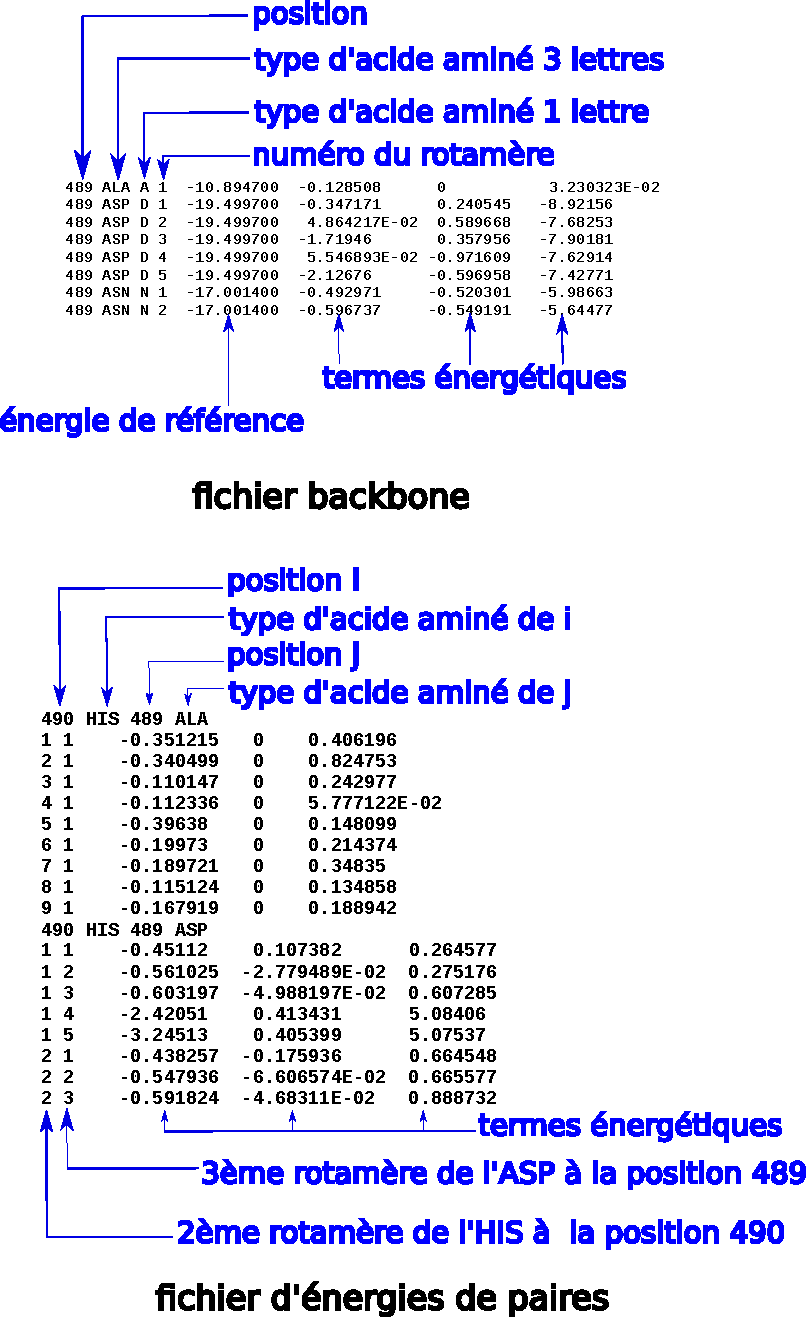
\includegraphics[width=12cm]{figure/inputener.pdf} 
     \end{tabular}     
     \caption{Les fichiers d'énergies en mode CASA}
\label{fig:CAenerfile}
   \end{figure}

   \begin{figure}[!htbp]
     \centering
     \begin{tabular}{c}
       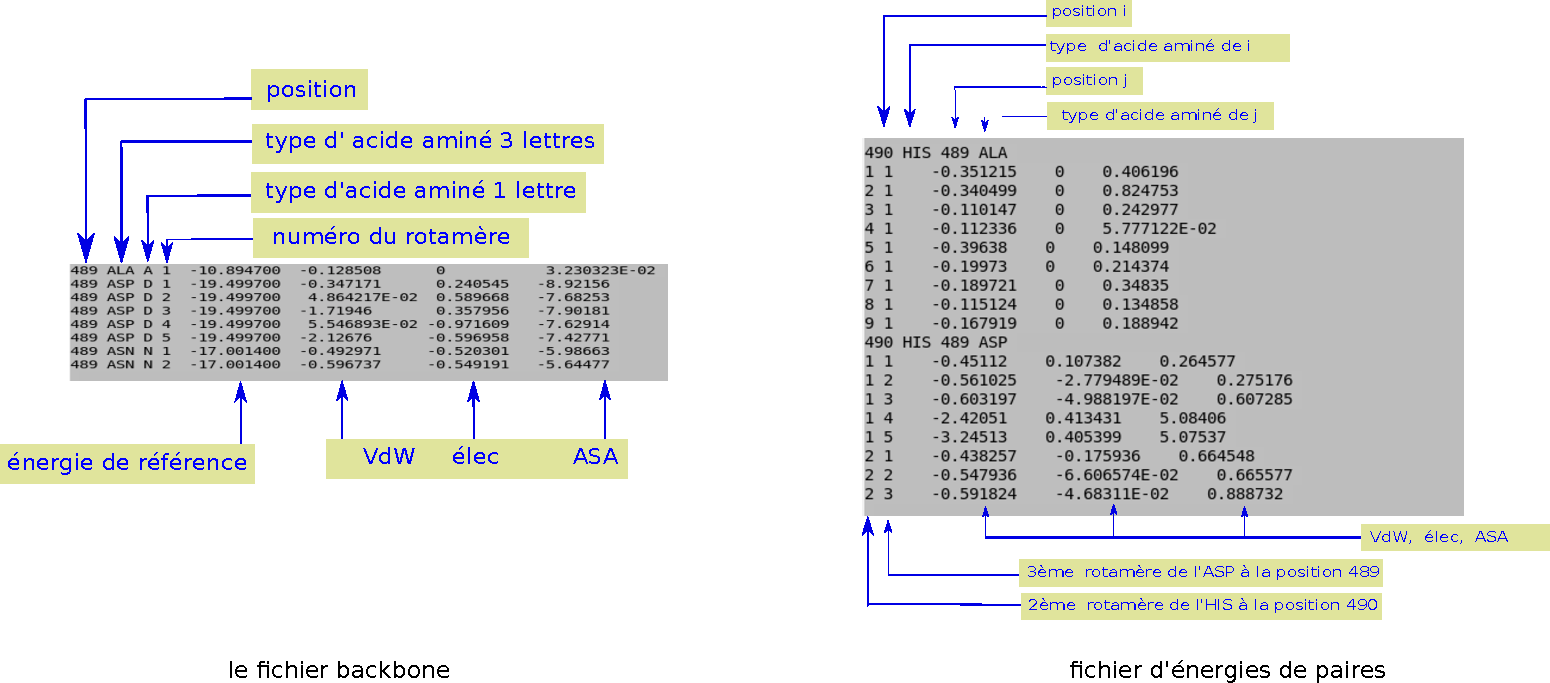
\includegraphics[width=16cm]{figure/inputenerFDB.pdf} 
     \end{tabular}     
     \caption{Les fichiers d'énergies en mode GB/FDB}
\label{fig:GBenerfile}
   \end{figure} 
   
\section{Configuration de l'exploration}
L'étape suivante est l'exploration de l'espace. Elle s'effectue avec le programme proteus écrit en C. Ce programme se contrôle par un fichier de configuration de type XML sans imbrication de balise. Il y a actuellement près de quarante balises possibles, une partie est présentée table \vref{tab:balise_proteus}. Nous en détaillons quelques-unes ici. L'utilisateur peut choisir la méthode d'exploration entre MSD (\og Multistart Steepest Descent heuristic \fg), MC/REMC ou le champ moyen. Pour le MSD, il peut paramétrer le nombre de cycles et le nombre de passages sur la séquence, voir section \vref{MSD}.
Pour le MC/REMC, le fichier de configuration détermine le nombre de marcheurs, la taille de chaque trajectoire et la période de \og swap \fg, c'est-à-dire la période, en nombre de pas, à laquelle une tentative d'échange de répliques est effectuée, voir \vref{REMC_move}. Si elle est non nulle, l'exploration est de type REMC.

Pour contrôler les déplacements des marcheurs REMC, il existe 
\begin{itemize}
\item cinq  balises pour définir les déplacements
\item une balise qui définit un voisinage de chaque position, utilisé en cas de double déplacement.
\end{itemize}
Il est possible de réduire l'espace des états que peut prendre une séquence-conformation. Les explications sont en \ref{sub:restric}.  Il existe deux balises pour définir un système de groupes et déclarer une fonction de score. Elles permettent de définir une optimisation non plus uniquement du type de l'équation \ref{deltaG}, mais répondant à un ensemble de problématiques plus large. Nous expliquons ce système en \vref{sub:group}.
 
    \begin{table}[!htbp]
      \centering

      \begin{tabular}{|p{0.2\linewidth}|p{0.32\linewidth}|p{0.48\linewidth}|}

        \hline
        Type   & nom & Description \\
        \hline
          méthode  d'exploration & Mode &  détermine  le mode d'exécution: HEURISTIC(MSD), MONTECARLO, MEANFIELD et POSTPROCESS  \\  \hline    
                        & Trajectory\_Length  &  la longueur de la trajectoire MC ou REMC\\  \cline{2-3}
        nombre de pas & Trajectory\_Number  &  le nombre de trajectoires  MC ou REMC  \\  \cline{2-3}
                        & Cycle\_Number  &    le nombre de cycles en mode HEURISTIC   \\ \cline{2-3}  
                        & Sequence\_Pass\_Number  &  le nombre maximum d'itérations sur  la structure à chaque cycle HEURISTIC    \\ \hline  

        fonction d'énergie &  Optimization\_Configuration &   définition de la fonction d'énergie\\               \cline{2-3}
                        &  Group\_definition &   groupes  d'énergies et d'énergies d'interactions\\  \hline  
        restrictions de l'espace de  séquences-rotamères & Space\_Constraints   &  restreint les états pouvant être visités \\ \hline                
                         
     paramètre  & Temperature & attribue les températures aux marcheurs REMC  \\          \hline     
                         & Random\_Generator &  le générateur de nombre aléatoire de la \og GNU Scientific Library \fg \\ \cline{2-3}
                         & Rot\_Proba &  probabilité d'avoir un changement de rotamère à chaque pas \\              
        configuration    & Rot\_Rot\_Proba &  probabilité d'avoir un double changement de rotamères à chaque pas\\          
        Monte Carlo      & Mut\_Proba &  ... \\              
                         & Mut\_Mut\_Proba & ... \\              
                         & Mut\_Rot\_Proba & ... (ancienne version de Proteus)\\             \cline{2-3}  
                         & Position\_Weights  & probabilité de tirage de chaque position, lors du premier choix\\  
                         & Step\_Definition\_Proba  & probabilité de changer un rotamère ou un type d'acide aminé\\   \cline{2-3}
        
                         & Neighbor\_Threshold & Définit la taille des voisinages.\\   \hline
        
                         & Fasta\_File & le nom du fichier produit par POSTPROCESS\\    \cline{2-3}             
        entrées/sorties     & Seq\_Output\_File & le nom  du fichier de séquences produit par HEURISTIC ou MONTECARLO\\    \cline{2-3}             
                         & Energy\_Output\_File & le nom du fichier d'énergie produit par HEURISTIC ou MONTECARLO\\   \hline              

      \end{tabular} 

      \caption{une partie des balises possibles du fichier de configuration de proteus}      

      \label{tab:balise_proteus}
      

    \end{table}
    

\subsection{Les déplacements Monte Carlo}
\label{sub:MC_move}  
Dans l'algorithme de Metropolis, il est nécessaire de définir une probabilité de sélectionner un état $B$ lorsque le système est dans l'état $A$. Pour proteus, une transition se définit par des modifications à certaines positions de la séquence-conformation courante. Il y a deux classes de modifications élémentaires: une mutation et un changement de rotamère. Cinq balises permettent de définir des probabilités associées à ces modifications: \\
\verb!<Rot_Proba>! \\
\verb!<Mut_Proba>! \\
\verb!<Rot_Rot_Proba>! \\
\verb!<Mut_Rot_Proba>! \\
\verb!<Mut_Mut_Proba>!  \\
Chacune prend en paramètre une valeur comprise entre $0$ et $1$. Les deux premières fixent la probabilité des deux modifications élémentaires. Les trois autres fixent la probabilité de modifier deux positions simultanément, au cours d'un même pas Monte-Carlo. Le choix d'une première position à modifier se fait par tirage équiprobable sur l'ensemble des positions. Le choix de la seconde position se fait par tirage dans le voisinage de la première. Deux positions $i$ et $j$ sont voisines s'il existe un rotamère $r_i$ de $i$ et un rotamère $r_j$ de $j$ tels que:
\begin{displaymath}
  \label{eq:voisin}
 | E(r_i,r_j) | > S
\end{displaymath} 
avec $S$ le seuil donné par l'utilisateur dans la balise \verb!<Neighbor_Threshold>!. Le voisinage d'une position $i$ est l'ensemble de ses voisins. Ce système de déplacements MC a été revu pendant ma thèse, voir section \vref{sec:newmove}.

\subsection{Restriction de l'espace séquence-conformation}
\label{sub:restric}
Dans proteus, l'espace des états possibles se définit par le contenu du fichier \og backbone \fg. Cependant, l'utilisateur peut restreindre cet espace de la façon suivante:\\
\verb!<Space_Constraints>! \\
\verb!489  LYS TRP! \\
\verb!490  ASN ARG{1,8,12}! \\
\verb!</Space_Constraints>! \\
Cela signifie qu'à la position 489, seuls les types LYS et TRP sont possibles et qu'à la position 490, les types ASN et ARG sont seuls possibles et que pour ARG seuls les rotamères 1, 8  et 12 sont autorisés (selon l'indexation fournie dans le fichier \og backbone \fg). Cette balise permet aussi d'autres classes de restrictions exposées plus loin.

\subsection{Définition de la fonction de score }

Le cycle thermodynamique figure \ref{fig:cycleThermo} peut être adapté pour exprimer d'autres problématiques que celle de la recherche de séquences stables. C'est le cas des calculs de $pK_a$ qui dépendent d'une énergie libre de protonation. Le  problème de la reconnaissance d'un ligand peut également être traité, par un critère d'affinité ou de spécificité. Le critère d'affinité se base sur le cycle thermodynamique  \ref{fig:cycleThermoLigand} qui permet d'écrire l'équation:
\begin{equation}
   \label{deltaG2}
\Delta \Delta G = (G(P\!:\!L_2)- G(P\!:\!L_1)) - (G(L_2) - G(L_1))
\end{equation}  
avec $P$ la protéine, $L_1$ et $L_2$ deux ligands et $P\!:\!L_i$ un complexe protéine-ligand. 

   \begin{figure}[!htbp]
     \centering
       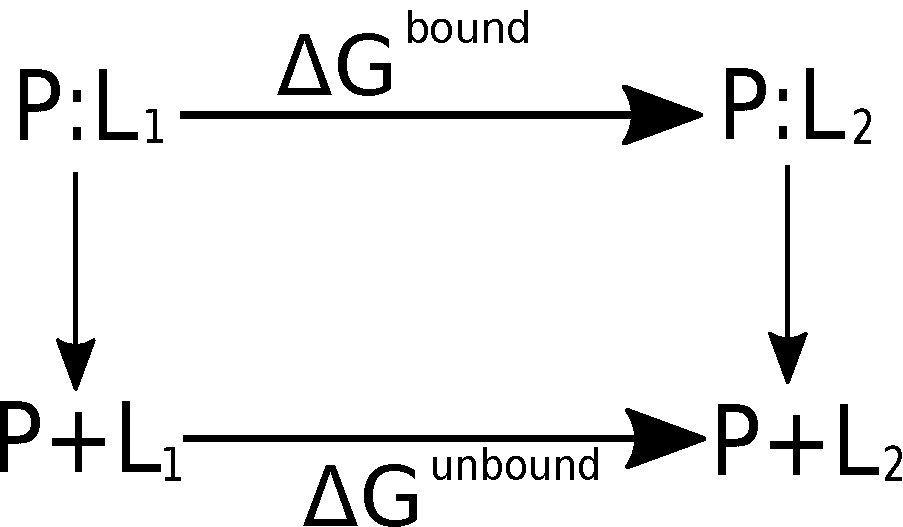
\includegraphics[width=6cm]{figure/cycleThermoLigand.pdf} 
     \caption{Cycle thermodynamique qui définit l'affinité.}
\label{fig:cycleThermoLigand}
   \end{figure}
Le critère de spécificité combine une augmentation du poids d'un ligand et la réduction du poids d'un autre. En effet, Proteus permet la décomposition des équations \ref{deltaG} et \ref{deltaG2} en contributions intramoléculaire et intermoléculaire. De plus, il autorise une pondération des différents termes et permet de dupliquer des parties du système. Cela permet également des optimisations simultanées de deux conformations à séquences identiques, mais non fixées. Un exemple est donnée avec la déclaration de deux balises suivantes:\\
\verb!<Group_Definition>!\\
\verb!prot 5-611!\\
\verb!lig 901!\\
\verb!</Group_Definition>!\\
et\\
\verb!<Optimization_Configuration>!\\
\verb!m(0.6prot~lig+0.2lig+0.2prot)!\\
\verb!</Optimization_Configuration>!\\
Nous détaillons en annexe la façon dont ce dispositif fonctionne.

\section{Les fichiers de sortie}
\label{proteusIO}
Dans le mode HEURISTIC (algorithme MSD), proteus produit en sortie deux fichiers. Un fichier de conformations-séquences donne à chaque ligne, la meilleure séquence-conformation d'un cycle, son énergie au sens de la fonction de score, le nombre de passages sur la séquence nécessaire à son obtention, voir la section \vref{MSD}. Le second fichier donne la fonction de score et l'énergie de chaque groupe ou interaction de groupe utilisée, ceci pour chacune des séquences-conformations du premier fichier. Le lien entre les deux fichiers se fait par l'identifiant unique de résultats situé dans la première colonne des deux fichiers.

Dans le mode MONTECARLO (algorithmes MC et REMC), sont produits un fichier de conformations-séquences et un fichier d'énergies par marcheur. Le format de ces fichiers est le même que celui du mode HEURISTIC, excepté pour le champ contenant le nombre de passages sur la séquence: ici, il est occupé par le nombre de pas pendant lequel le marcheur est resté dans la séquence-conformation avant un déplacement. La température est dans l'entête.

   \begin{figure}[!htbp]
     \centering 
     \begin{tabular}{cc}
       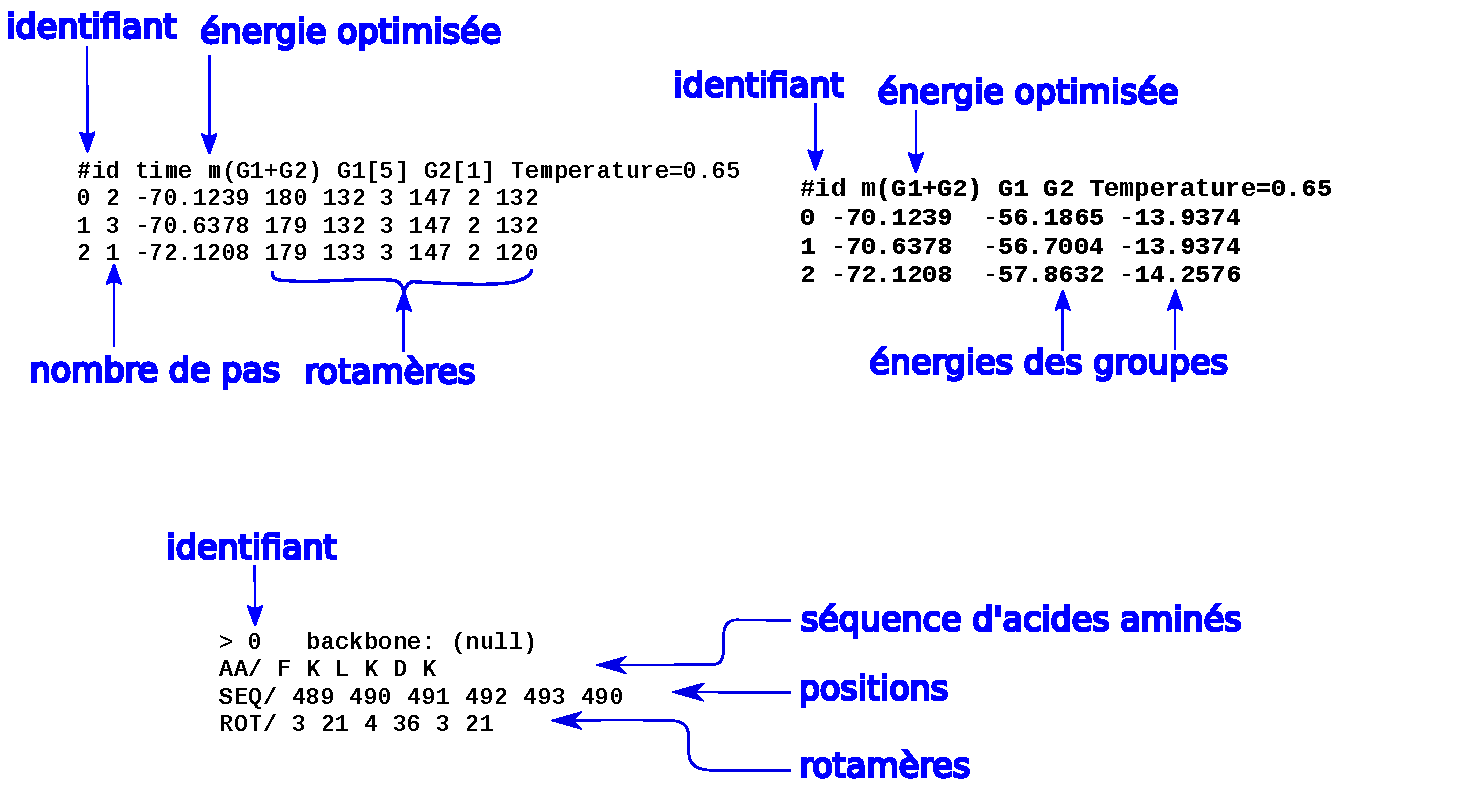
\includegraphics[width=18cm]{figure/output.pdf} &
     \end{tabular}
     
     \caption{\textbf{Les fichiers en sortie de proteus} en haut pour le mode MONTECARLO, en bas pour le mode POSTPROCESS}
\label{proteusoutput}
   \end{figure}

Dans les fichiers précédents, les séquences-conformations sont présentées sous forme de listes de nombres qui correspondent au nième rotamère de chaque position selon le fichier backbone. Le mode POSTPROCESS propose une conversion de ce format vers un format de type FASTA où apparaissent la séquence d'acides aminés, la liste des rotamères donnés par leur numéro et les positions PDB pour chaque séquence-conformation. Le format de ces fichiers est présenté à la figure \ref{proteusoutput}.

\section{Outils d'analyse de séquences}

Nous présentons maintenant les outils d'analyse que nous utilisons pour examiner la qualité de nos résultats.
\subsection{Superfamily/SCOP}
\label{sec:Superfamily}
Superfamily \cite{Madera04} comprend: 
\begin{itemize}
\item une base de données de modèles de Markov cachés, où chaque modèle représente une structure 3D d'un domaine de la classification SCOP \cite{Andreeva04}.
\item une série de scripts qui annotent les séquences données en entrée. Ici, nous utilisons uniquement l'association de chaque séquence au modèle SCOP le plus vraisemblable. 
\end{itemize}
Nous travaillons avec la version 1.75 et nous utilisons SAM (version 3.5) \cite{hughey95} et HMMER (version 3.0) \cite{HMMER}, deux outils de manipulation de modèles de Markov cachés pour la biologie recommandées par l'équipe de Superfamily. La base SCOP contient 15 438 modèles.

\subsection{Taux d'identité de séquences}

Soient $S$ et $N$ deux séquences d'acides aminés de même longueur $l$. Le taux d'identité $Id(S,N)$ de $S$ par rapport $N$ est égal au pourcentage de positions où l'acide aminé est identique dans $S$ et $N$:
\begin{equation}
Id(S,N) =\frac{1}{l}\sum_{1 \leqslant i \leqslant l} \mathds{1}(s_i,n_i) \times 100
\end{equation}
avec $s_i$ et $n_i$ l'acide animé en $i$ de $S$ et de $N$ respectivement, et $\mathds{1}(x,y)$ la fonction qui vaut $1$ lorsque $x=y$ et $0$ sinon. 
\subsection{Taux d'identité par position}
\label{TauxID}
Le taux d'identité d'un alignement $A_S$ à la position $i$ par rapport à une séquence $N$ de même longueur se définit comme:
\begin{equation}
Id(A_{S},i) = \frac{1}{m}\sum_{1\leqslant j \leqslant m} \mathds{1}(s_i^j,n_i) \times 100
\end{equation}
avec $m$ le nombre de séquences de $A_S$. Ce taux d'identité donne une mesure de la ressemblance entre un alignement et une séquence. Cela nous permet de comparer nos séquences calculées aux séquences naturelles de la famille de la native.  
\subsection{Alignements Pfam}
\label{sec:Align_Pfam}
La base de données Pfam (Protein families database) \cite{Punta12,Finn14} regroupe les domaines protéiques en familles. Chaque famille est représentée par des alignements multiples de séquences et des modèles de Markov cachés. Dans la suite, nous utilisons l'alignement \og seed \fg qui est un petit alignement de séquences naturelles représentatives. Il contient 45 séquences pour la famille PDZ. Nous utilisons également l'alignement \og RP55 \fg, qui se base sur l'alignement \og seed \fg et augmente le nombre de séquences grâce à des  modèles de Markov cachés construits à partir de \og seed \fg, jusqu'à contenir 12 255 séquences protéiques naturelles pour la famille PDZ.

\subsection{Score BLOSUM}

Pour tenir compte des ressemblances et des différences entre les acides aminés lors d'une substitution, nous avons besoin d'une matrice de coût. Nous utilisons les matrices BLOSUM40 et BLOSUM62 (BLOcks SUbstitution Matrix) \cite{Henikoff92} qui sont construites à partir de blocs d'alignement très conservés (plus de 40\% et 62\% d'identités respectivement). Le score BLOSUM d'une substitution calculé à partir de la fréquence de la mutation correspondante. À cela est ajouté un score de pénalités pour l'insertion d'un gap, c'est-à-dire un saut dans l'alignement.

On définit alors un score de similarité de deux séquences de même longueur comme la somme des scores BLOSUM62 sur toutes les positions. De même, le score de similarité d'un alignement par rapport à une séquence sera défini comme la moyenne des scores de similarité sur ensemble des séquences de l'alignement. Enfin, un score de similarité de deux ensembles de séquences alignés sera la moyenne des scores de similarité du premier ensemble par rapport aux séquences du second.  

\subsection{Similarité d'un ensemble à un alignement Pfam}
\label{SimPfam}
Afin de calculer un score de similarité d'un ensemble de séquences CPD par rapport à une famille Pfam, il faut commencer par aligner ces séquences avec l'alignement de la famille. Pour cela, nous utilisons le programme d'alignement BLAST \cite{Altschul97,Camacho08}. Il implémente une heuristique qui recherche puis étend les meilleurs alignements locaux. Nous procédons comme suit:
\begin{enumerate}[leftmargin=*]
\item La commande \verb!blastp! est utilisée avec comme base de données (paramètre \verb!-db!) l'alignement Pfam et comme séquence en entrée (paramètre \verb! -query!) la séquence native d'intérêt. 
\item Dans la sortie blast, la séquence qui produit l'alignement le plus significatif avec la native est collectée, notons-la $S_0$. 
\item L'alignement blast est alors utilisé pour positionner la native par rapport à $S_0$ et les gaps nécessaires pour aligner la native à $S_0$ sont ajoutés.
\item Le positionnement et les gaps sont alors appliqués tels quels aux séquences CPD.

\end{enumerate}

\subsection{Entropie par position}
\label{sec:Entropie}
Pour comparer la diversité des séquences CPD avec la diversité des séquences naturelles, nous utilisons l'entropie par position \cite{DurbinBK}, à partir de la formule:

\begin{equation} \label{eq:entropy}
  S_i = - \sum_{j=1}^6 f_j(i)lnf_j(i) \\
\end{equation} 
avec $f_j(i)$ la fréquence du type de résidu $j$ à la position $i$. Au lieu de distinguer les 20 types d'acides aminés, nous utilisons six classes de résidus, correspondant aux groupes suivants: \{L,V,I,M,C\}, \{F,Y,W\}, \{G\}, \{A,S,T,P\}, \{E,D,N,Q\} et \{K,R,H\}. Cette classification a été obtenue par un clustering de matrice BLOSUM62 et une analyse  des énergies de contact entre résidus dans les protéines \cite{Launay07}. Pour obtenir une mesure du nombre de types d'acides aminés apparaissant à une position, on utilise l'exponentielle de l'entropie par position $\exp(S)$ (qui varie de 1 à 6).  Cela correspond à un nombre moyen de classes échantillonnées par position. Par exemple, une valeur de 2 à une position particulière indique que les acides aminés de deux des six classes sont présents à cette position en moyenne au sein des séquences analysées. Ensuite, on moyenne cette valeur sur l'ensemble des résidus de la chaîne protéique. Une valeur moyenne globale de 2 indique qu'en moyenne, deux classes d'acides aminés sont présentes à n'importe quelle position.


\clearpage


%%% Local Variables:
%%% mode: latex
%%% TeX-master: "../these"
%%% End:
